\documentclass[10pt,a4paper,english]{article}
\usepackage[utf8]{inputenc}
\usepackage{amsmath}
\usepackage{amssymb}
\usepackage{pgfplots}
\usepackage{circuitikz}
\usetikzlibrary{intersections, pgfplots.fillbetween}
\usetikzlibrary{patterns}
\usetikzlibrary{shapes,snakes}
\pgfplotsset{compat=1.16}

\begin{document}

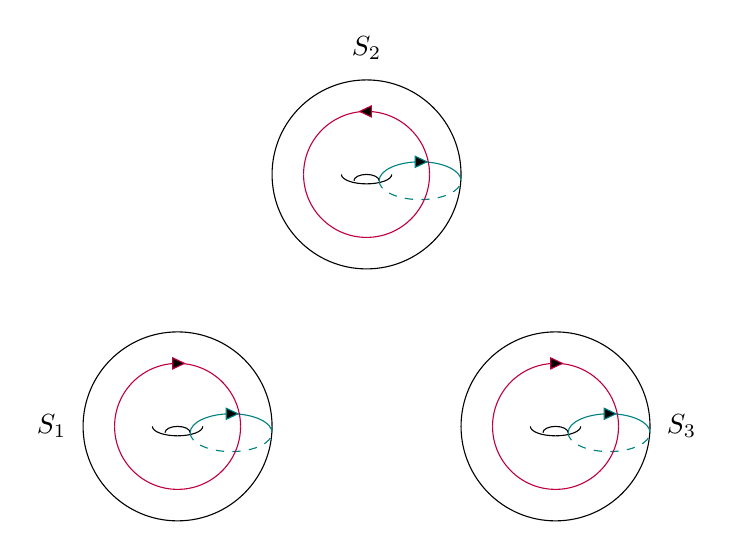
\begin{tikzpicture}[scale=0.8]
\draw (0,0) circle (1.5cm);
\draw (-0.4,0) arc (180:360:0.4cm and 0.15cm);
\draw (0.2,-0.1) arc (0:180:0.2cm and 0.1cm);
\draw [dashed, teal](0.2,-0.1) arc (180:360:0.65cm and 0.3cm);
\draw [teal](0.2,-0.1) arc (180:0:0.65cm and 0.3cm)
node[
    currarrow,
    pos=0.5, 
    xscale=1,
    sloped,
    scale=1] {};
\draw [purple] (-1,0) arc (180:0:1cm)
node[
    currarrow,
    pos=0.5, 
    xscale=1,
    sloped,
    scale=1] {};
\draw [purple] (-1,0) arc (180:360:1cm);
\begin{scope}[shift={(3,4)}]
\draw (0,0) circle (1.5cm);
\draw (-0.4,0) arc (180:360:0.4cm and 0.15cm);
\draw (0.2,-0.1) arc (0:180:0.2cm and 0.1cm);
\draw [dashed, teal](0.2,-0.1) arc (180:360:0.65cm and 0.3cm);
\draw [teal](0.2,-0.1) arc (180:0:0.65cm and 0.3cm)
node[
    currarrow,
    pos=0.5, 
    xscale=1,
    sloped,
    scale=1] {};
\draw [purple] (-1,0) arc (180:0:1cm)
node[
    currarrow,
    pos=0.5, 
    xscale=-1,
    sloped,
    scale=1] {};
\draw [purple] (-1,0) arc (180:360:1cm);
\end{scope}
\begin{scope}[shift={(6,0)}]
\draw (0,0) circle (1.5cm);
\draw (-0.4,0) arc (180:360:0.4cm and 0.15cm);
\draw (0.2,-0.1) arc (0:180:0.2cm and 0.1cm);
\draw [dashed, teal](0.2,-0.1) arc (180:360:0.65cm and 0.3cm);
\draw [teal](0.2,-0.1) arc (180:0:0.65cm and 0.3cm)
node[
    currarrow,
    pos=0.5, 
    xscale=1,
    sloped,
    scale=1] {};
\draw [purple] (-1,0) arc (180:0:1cm)
node[
    currarrow,
    pos=0.5, 
    xscale=1,
    sloped,
    scale=1] {};
\draw [purple] (-1,0) arc (180:360:1cm);
\end{scope}
\node (a) at (-2,0) {$S_{1}$};
\node (a) at (3,6) {$S_{2}$};
\node (a) at (8,0) {$S_{3}$};
\end{tikzpicture}

\end{document}